\documentclass[fleqn]{beamer}
\usepackage[spanish]{babel}

\usepackage{amsmath,amssymb}
\usepackage{graphicx}
\usepackage{dirtytalk}

\DeclareMathOperator*{\argmin}{arg\,min}

% vertical separator macro
\newcommand{\vsep}{
  \column{0.0\textwidth}
    \begin{tikzpicture}
      \draw[very thick,black!10] (0,0) -- (0,7.3);
    \end{tikzpicture}
}

% More space between lines in align
\setlength{\mathindent}{0pt}

% Beamer theme
\usetheme{ZMBZFMK}
\usefonttheme[onlysmall]{structurebold}
\mode<presentation>
%\setbeamercovered{transparent=10}

% align spacing
\setlength{\jot}{0pt}


\AtBeginSection[]
{
  \begin{frame}
    \frametitle{Tabla de contenidos}
    \tableofcontents[currentsection]
  \end{frame}
}


% Only the first Slide
\title{BASS como modelo base para optimización Bayesiana}
\author{Adrian Tame Jacobo}
\institute[Instituto Tecnológico Autónomo de México]{ Temas Selectos de Estadística }
\date{\today}


% Portada
\begin{document}
\begin{frame}
  \titlepage
\end{frame}

\section{Optimización Bayesiana}
\begin{frame}
  \frametitle{Introducción}
  Buscamos resolver el problema $$\max_{x \in A} f(x), $$
  donde: \begin{itemize}
      \item No tenemos información de las derivadas de $f$, ni información sobre su linealidad, concavidad, etc. La llamamos una función \say{caja negra}.
      \item Tenemos que si $x \in \mathbb{R}^d$, entonces $d \lesssim 20$. 
      \item \textit{La función} $f$ \textit{es continua}. 
      \item $f$ es difícil de evaluar.
  \end{itemize}
\end{frame}

\begin{frame}
  \frametitle{Procesos Gausianos}
  Sean $x_1, x_2, \ldots, x_k \in A$ puntos en los que evaluamos la función $f$. Sea $[f(x_1), \ldots, f(x_k)]$ un vector de estas evaluaciones. 
  \newline \\
  La distribución resultante o proceso Gausiano asociado sería entonces: 
  $$f(x_{1:k}) \sim \mathcal{N}(\mu_0(x_{1:k}), \Sigma_0(x_{1:k}, x_{1:k})).$$
  
  \begin{figure}[h]
    \centering
    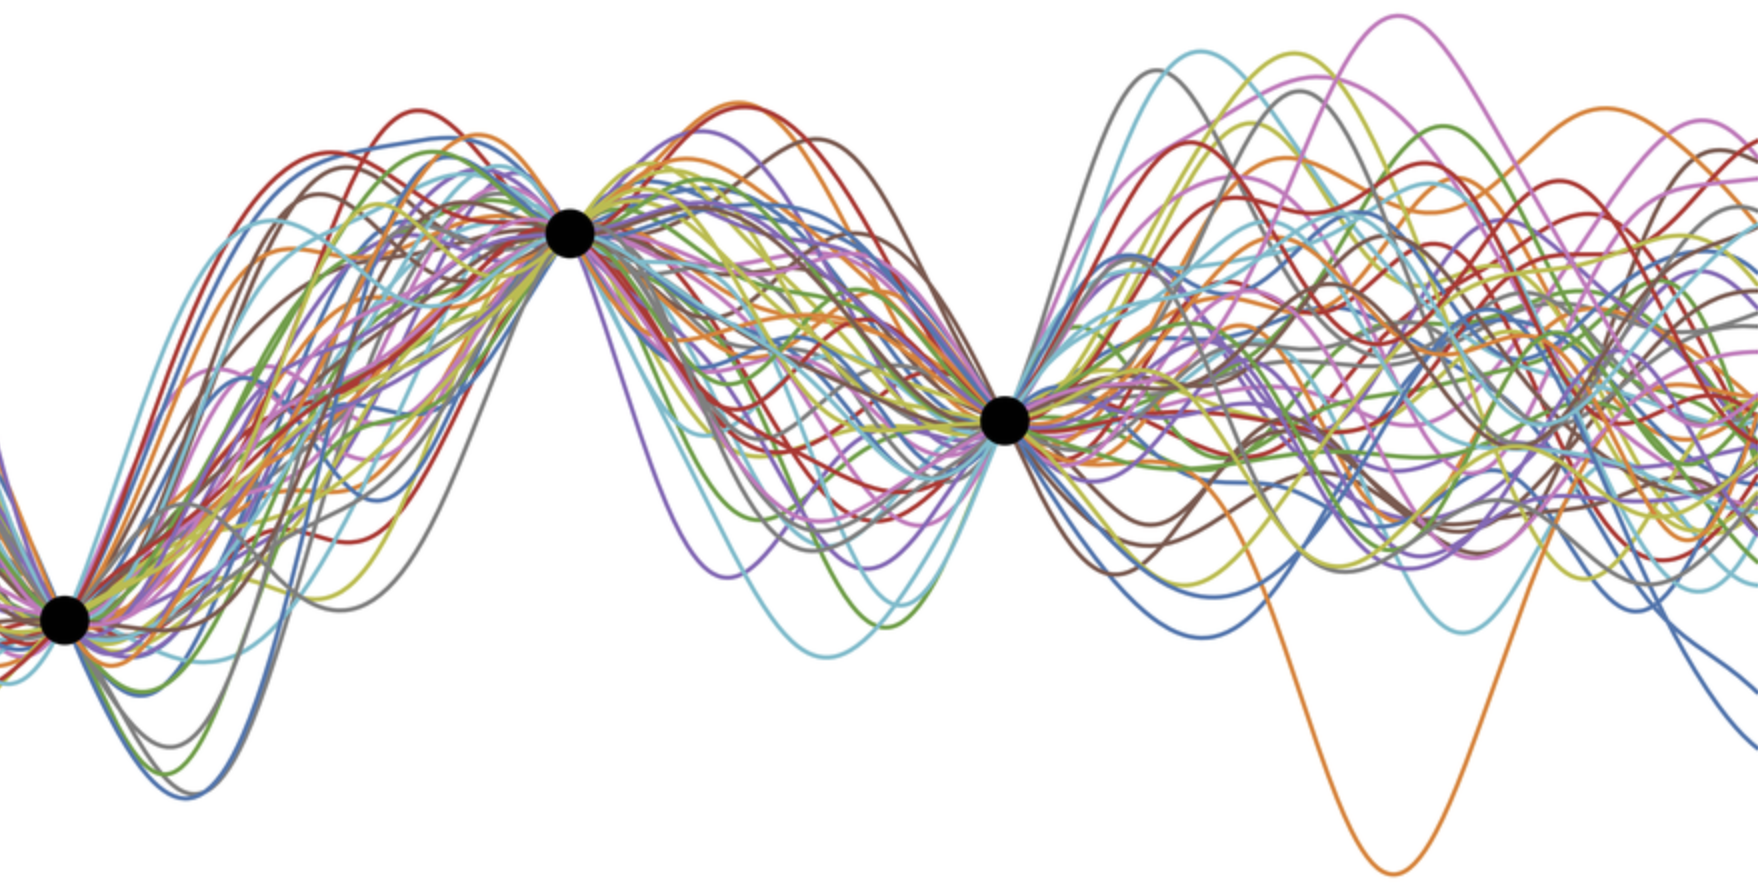
\includegraphics[width=0.5\textwidth]{Figures/gp1.png}
    \label{fig:mesh1}
  \end{figure}
\end{frame}

\begin{frame}
  \frametitle{Actualización de posterior}
  \begin{figure}[h]
    \centering
    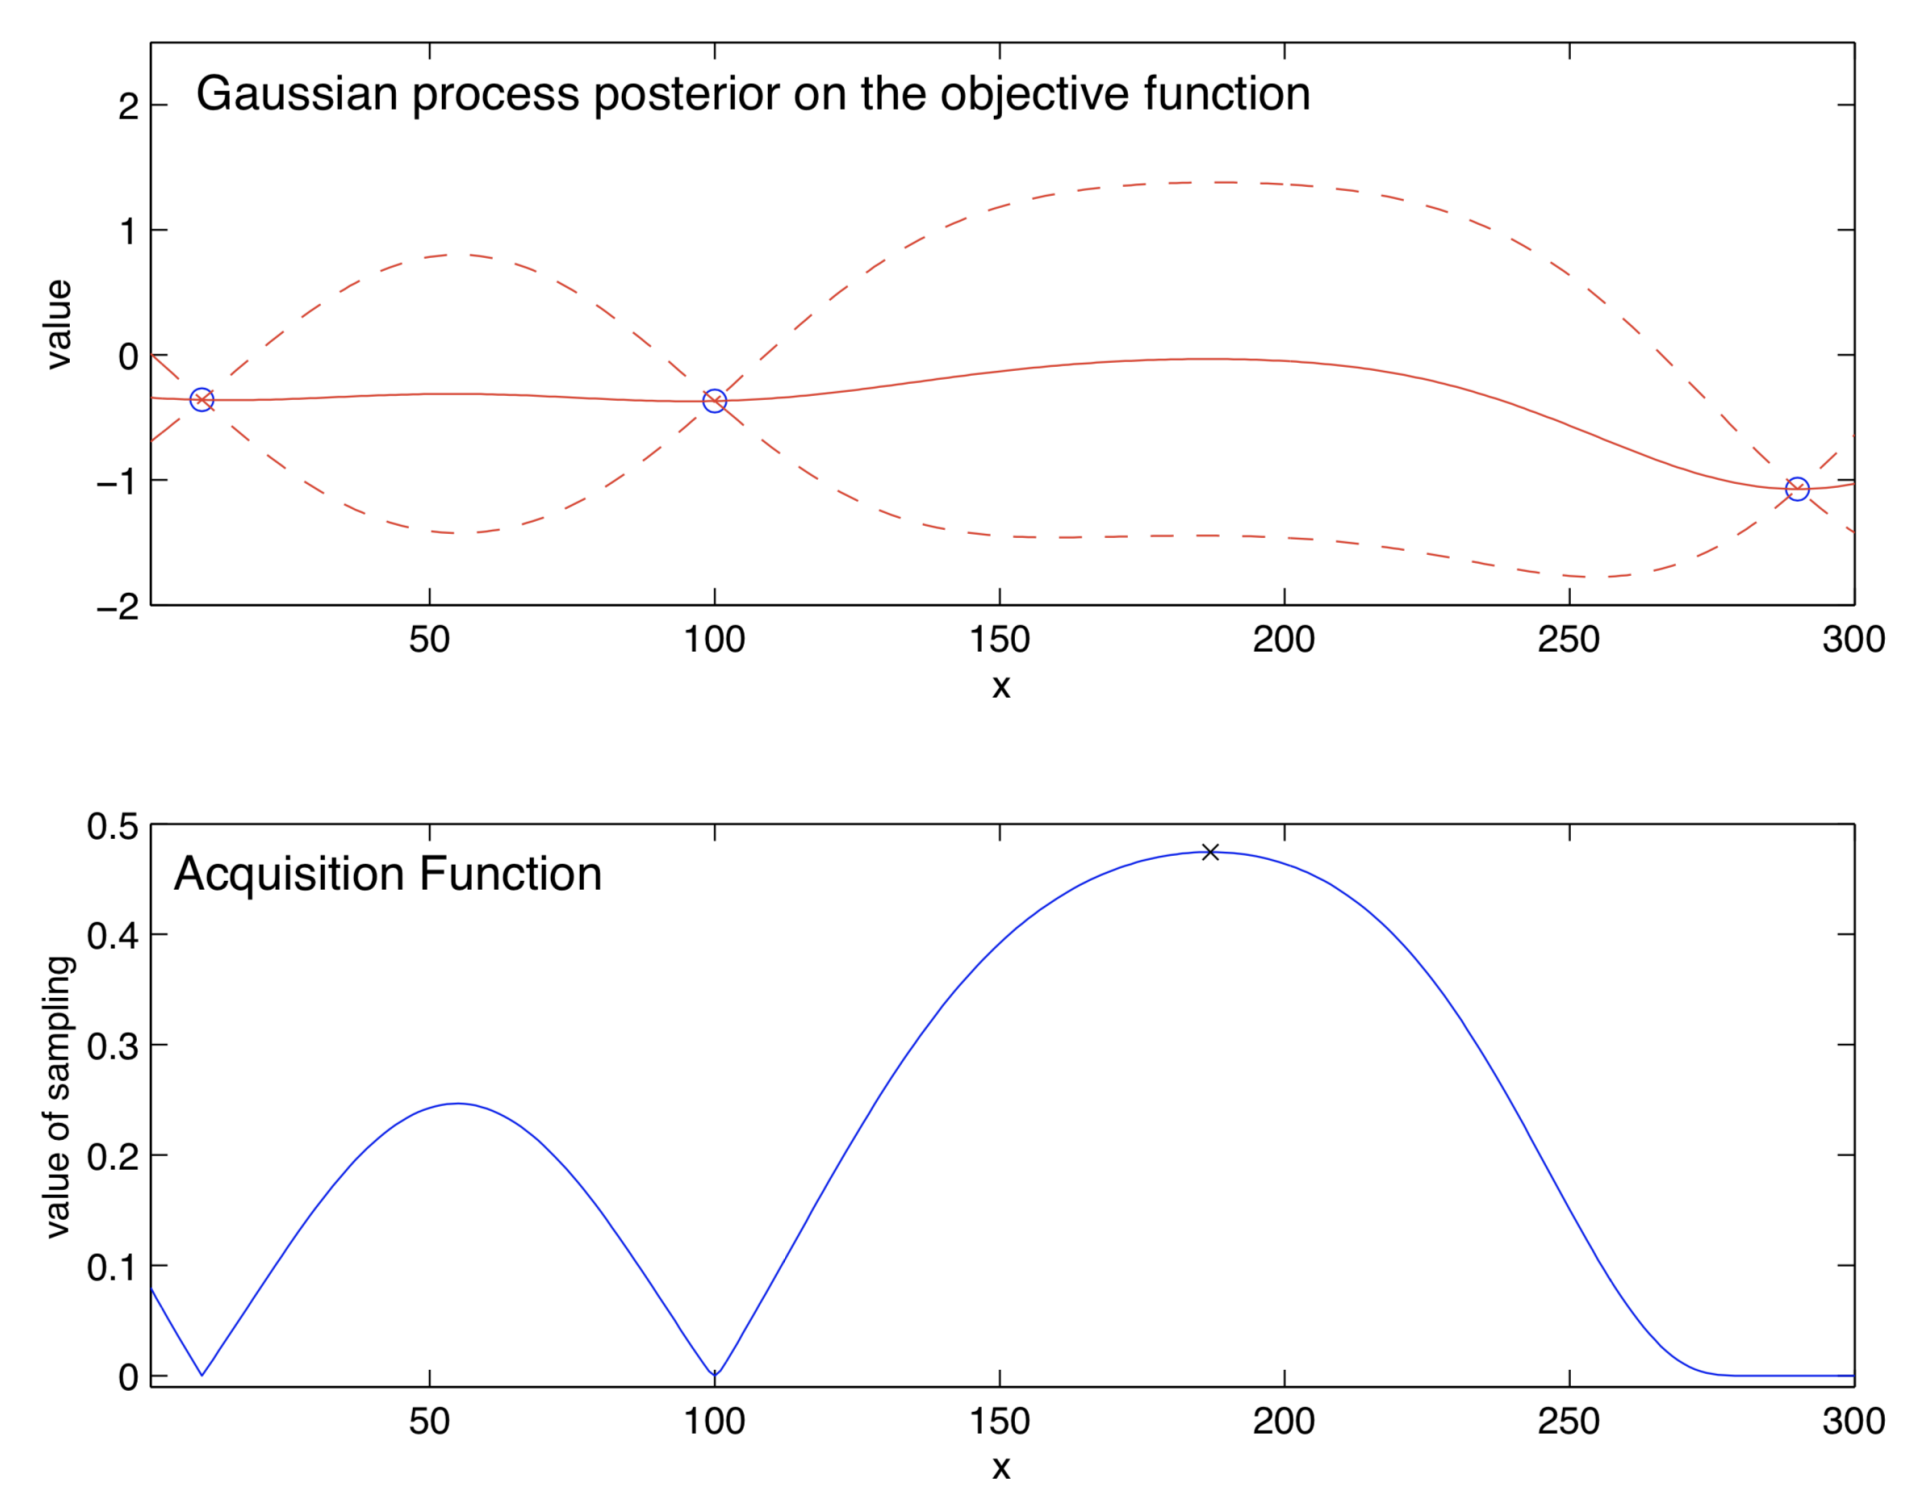
\includegraphics[width=0.75\textwidth]{Figures/acq.png}
    \label{fig:acq}
  \end{figure}
\end{frame}

\begin{frame}
  \frametitle{Algoritmo}
  \begin{figure}[h]
    \centering
    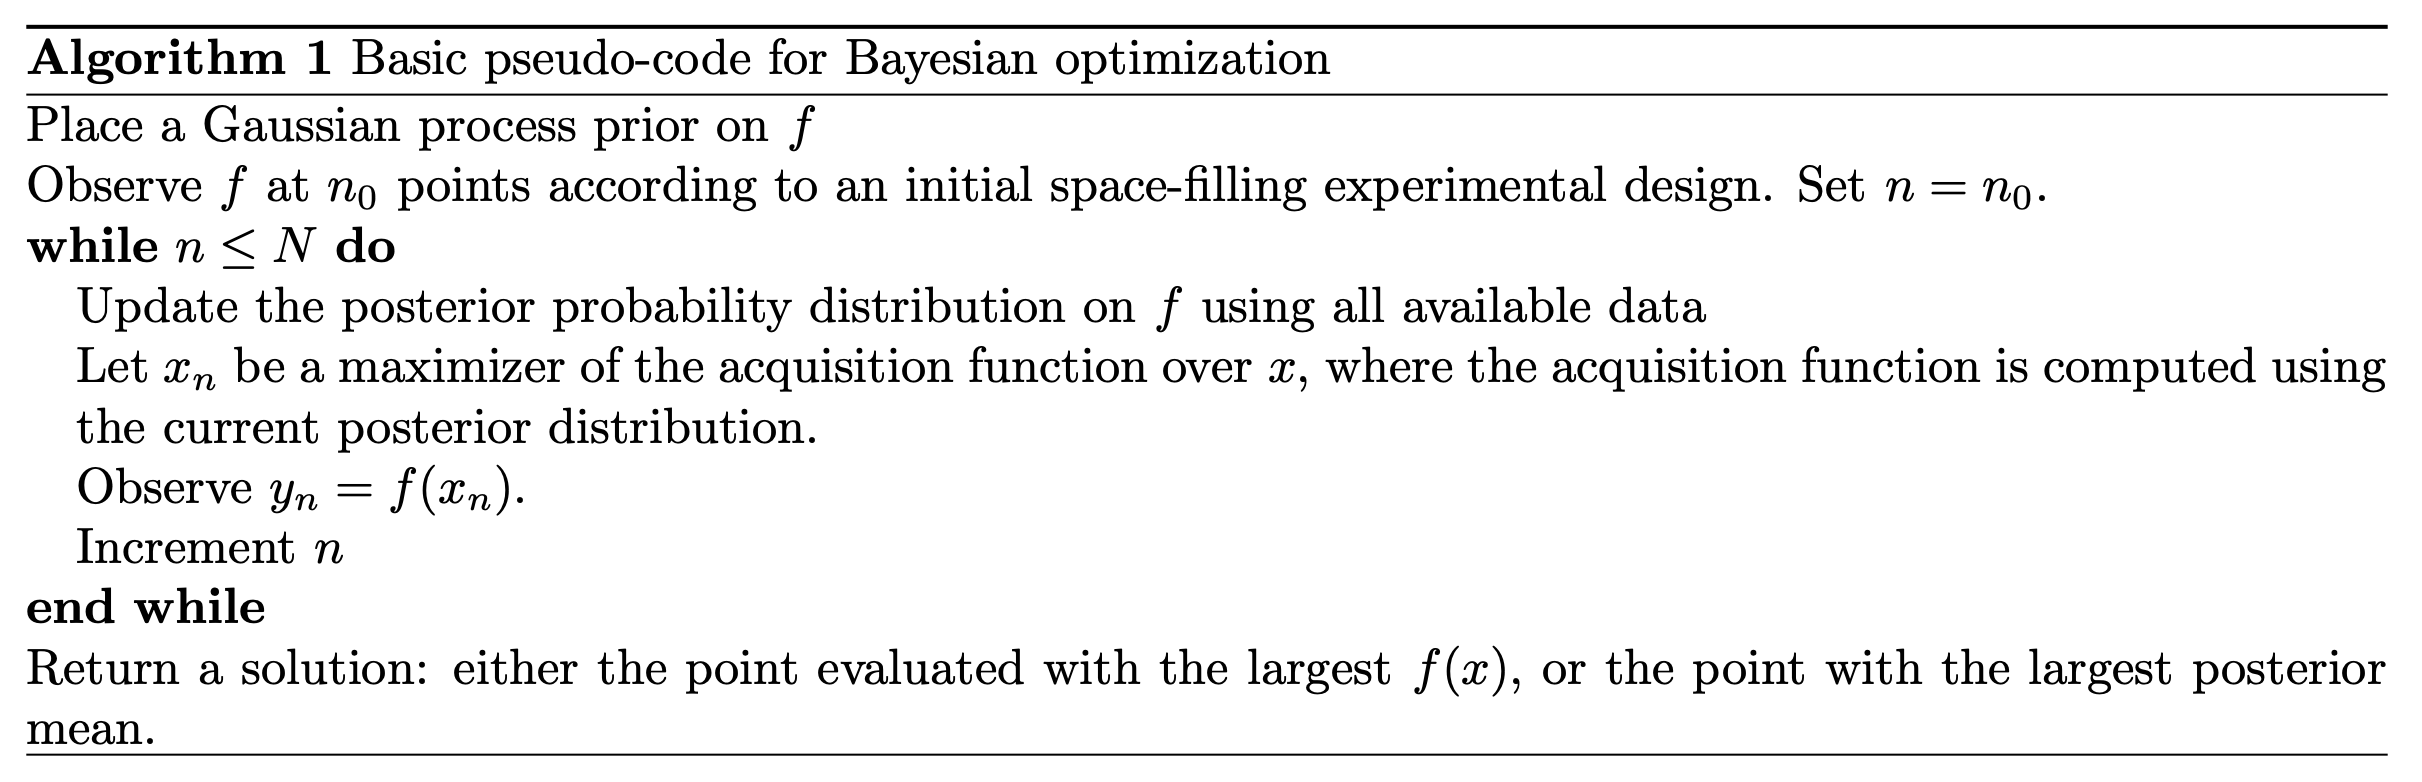
\includegraphics[width=1\textwidth]{Figures/algoritmo.png}
    \label{fig:algo}
  \end{figure}
\end{frame}

\begin{frame}
  \frametitle{Posterior y probabilidad de mejora}
  \begin{figure}[h]
    \centering
    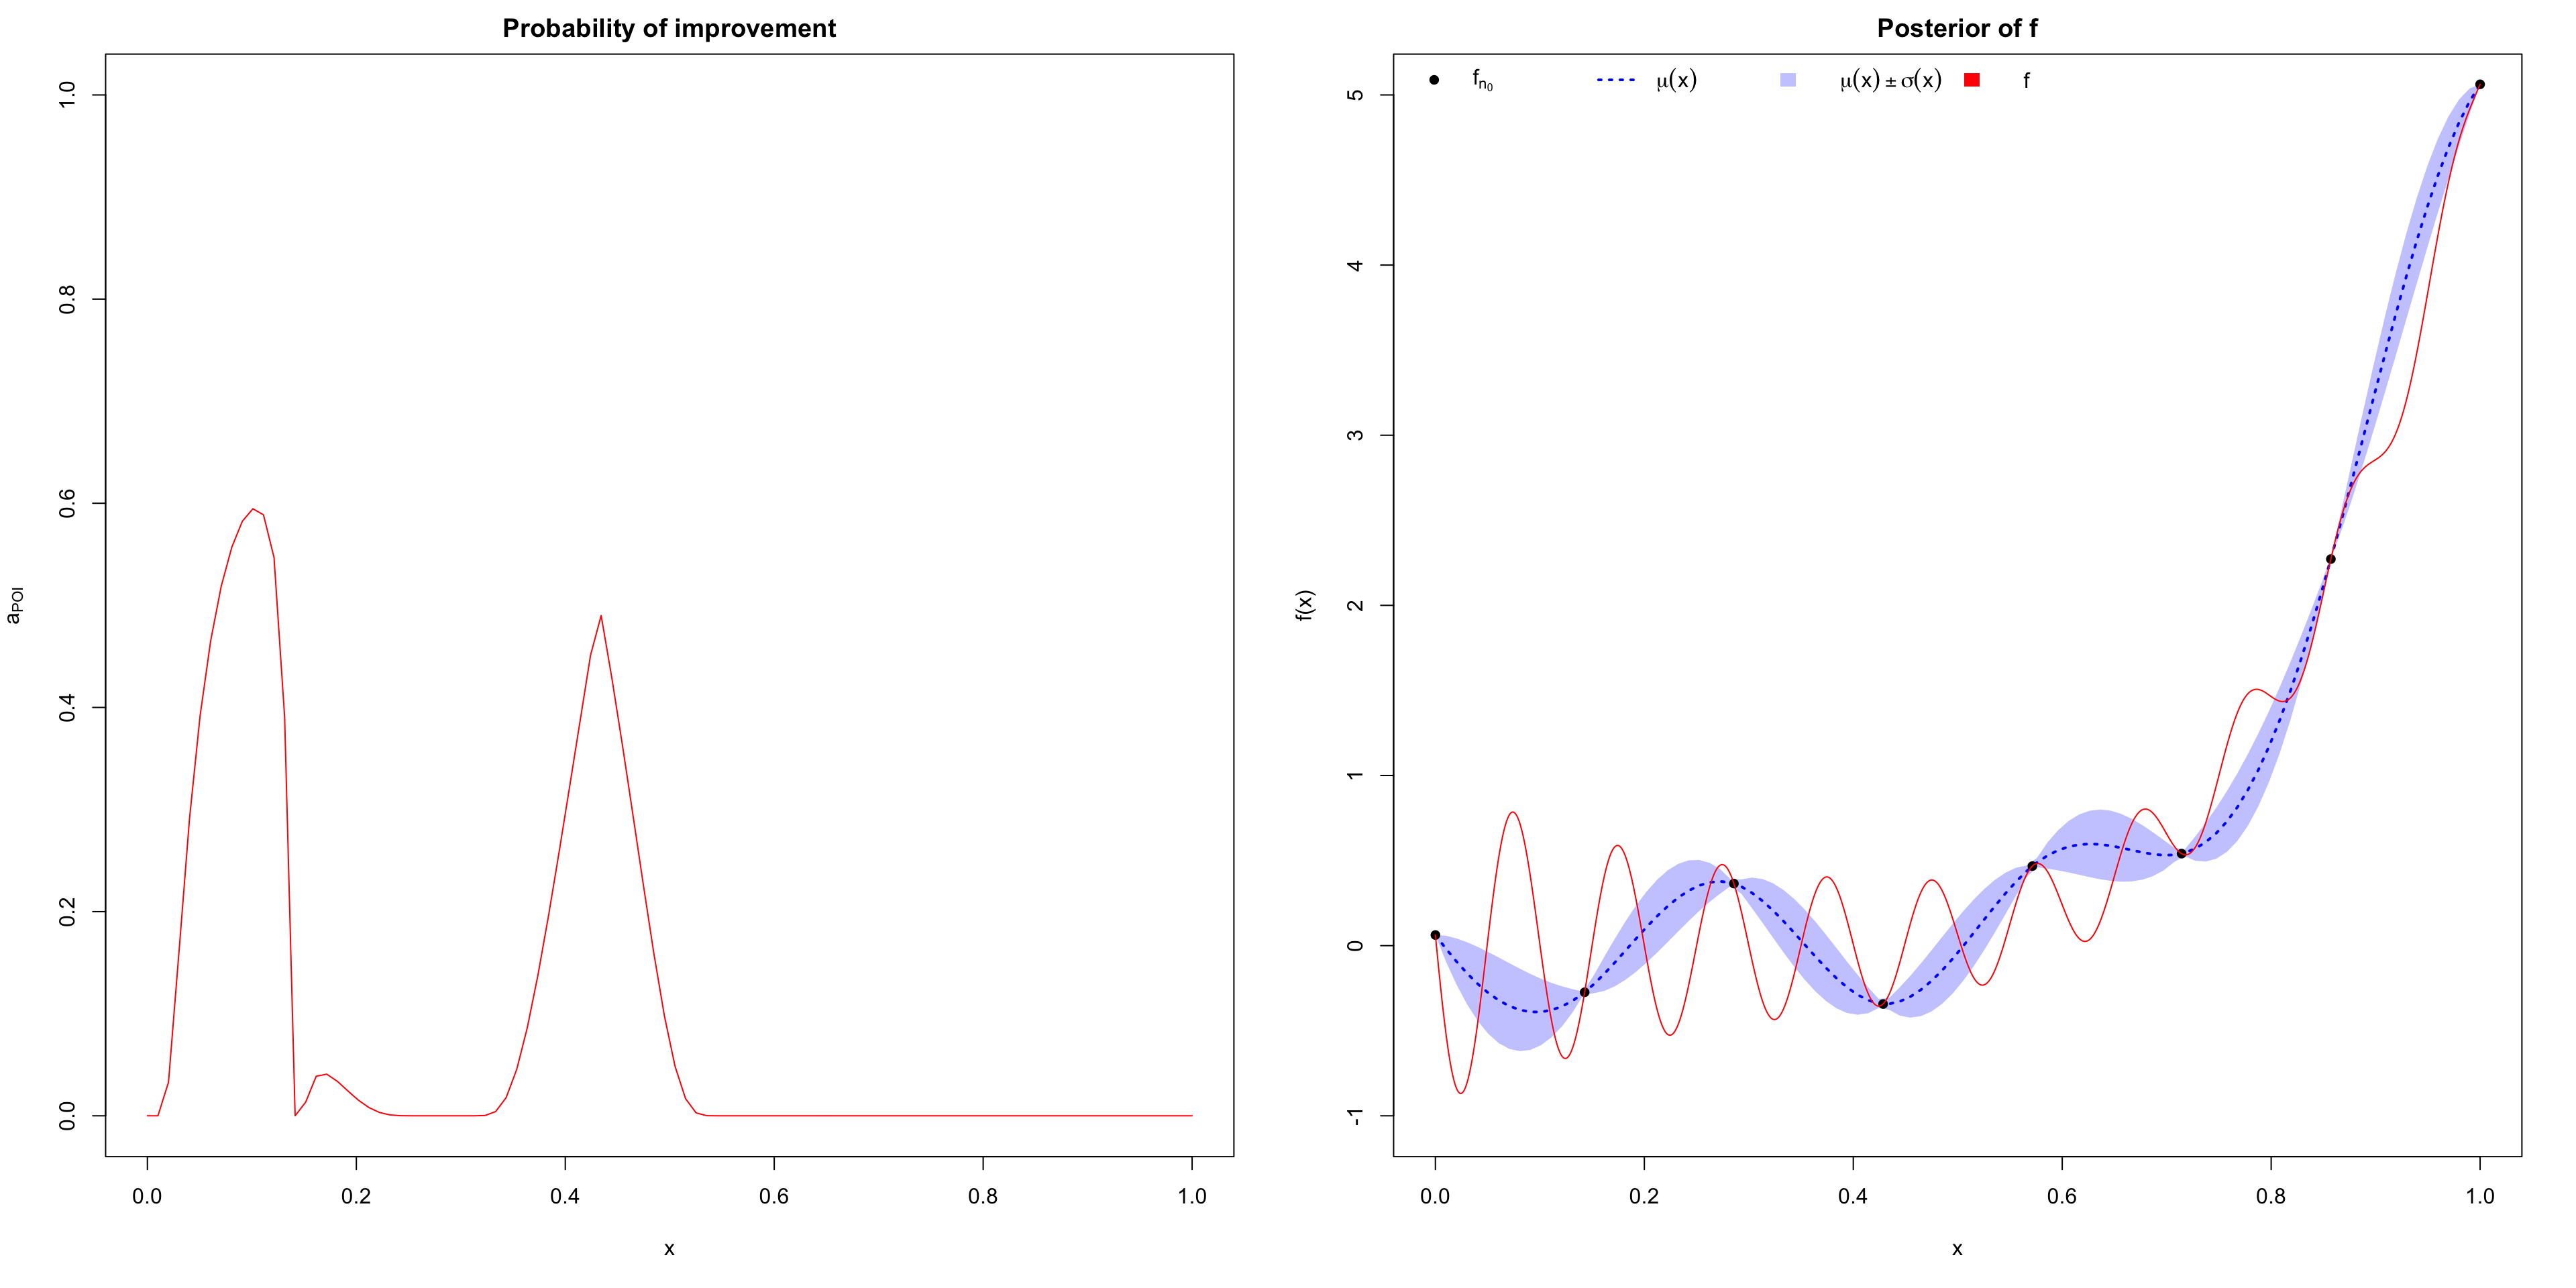
\includegraphics[width=1\textwidth]{Figures/ProbImprove.png}
    \label{fig:probimprove}
  \end{figure}
\end{frame}

\begin{frame}
  \frametitle{Después de 45 iteraciones}
  \begin{figure}[h]
    \centering
    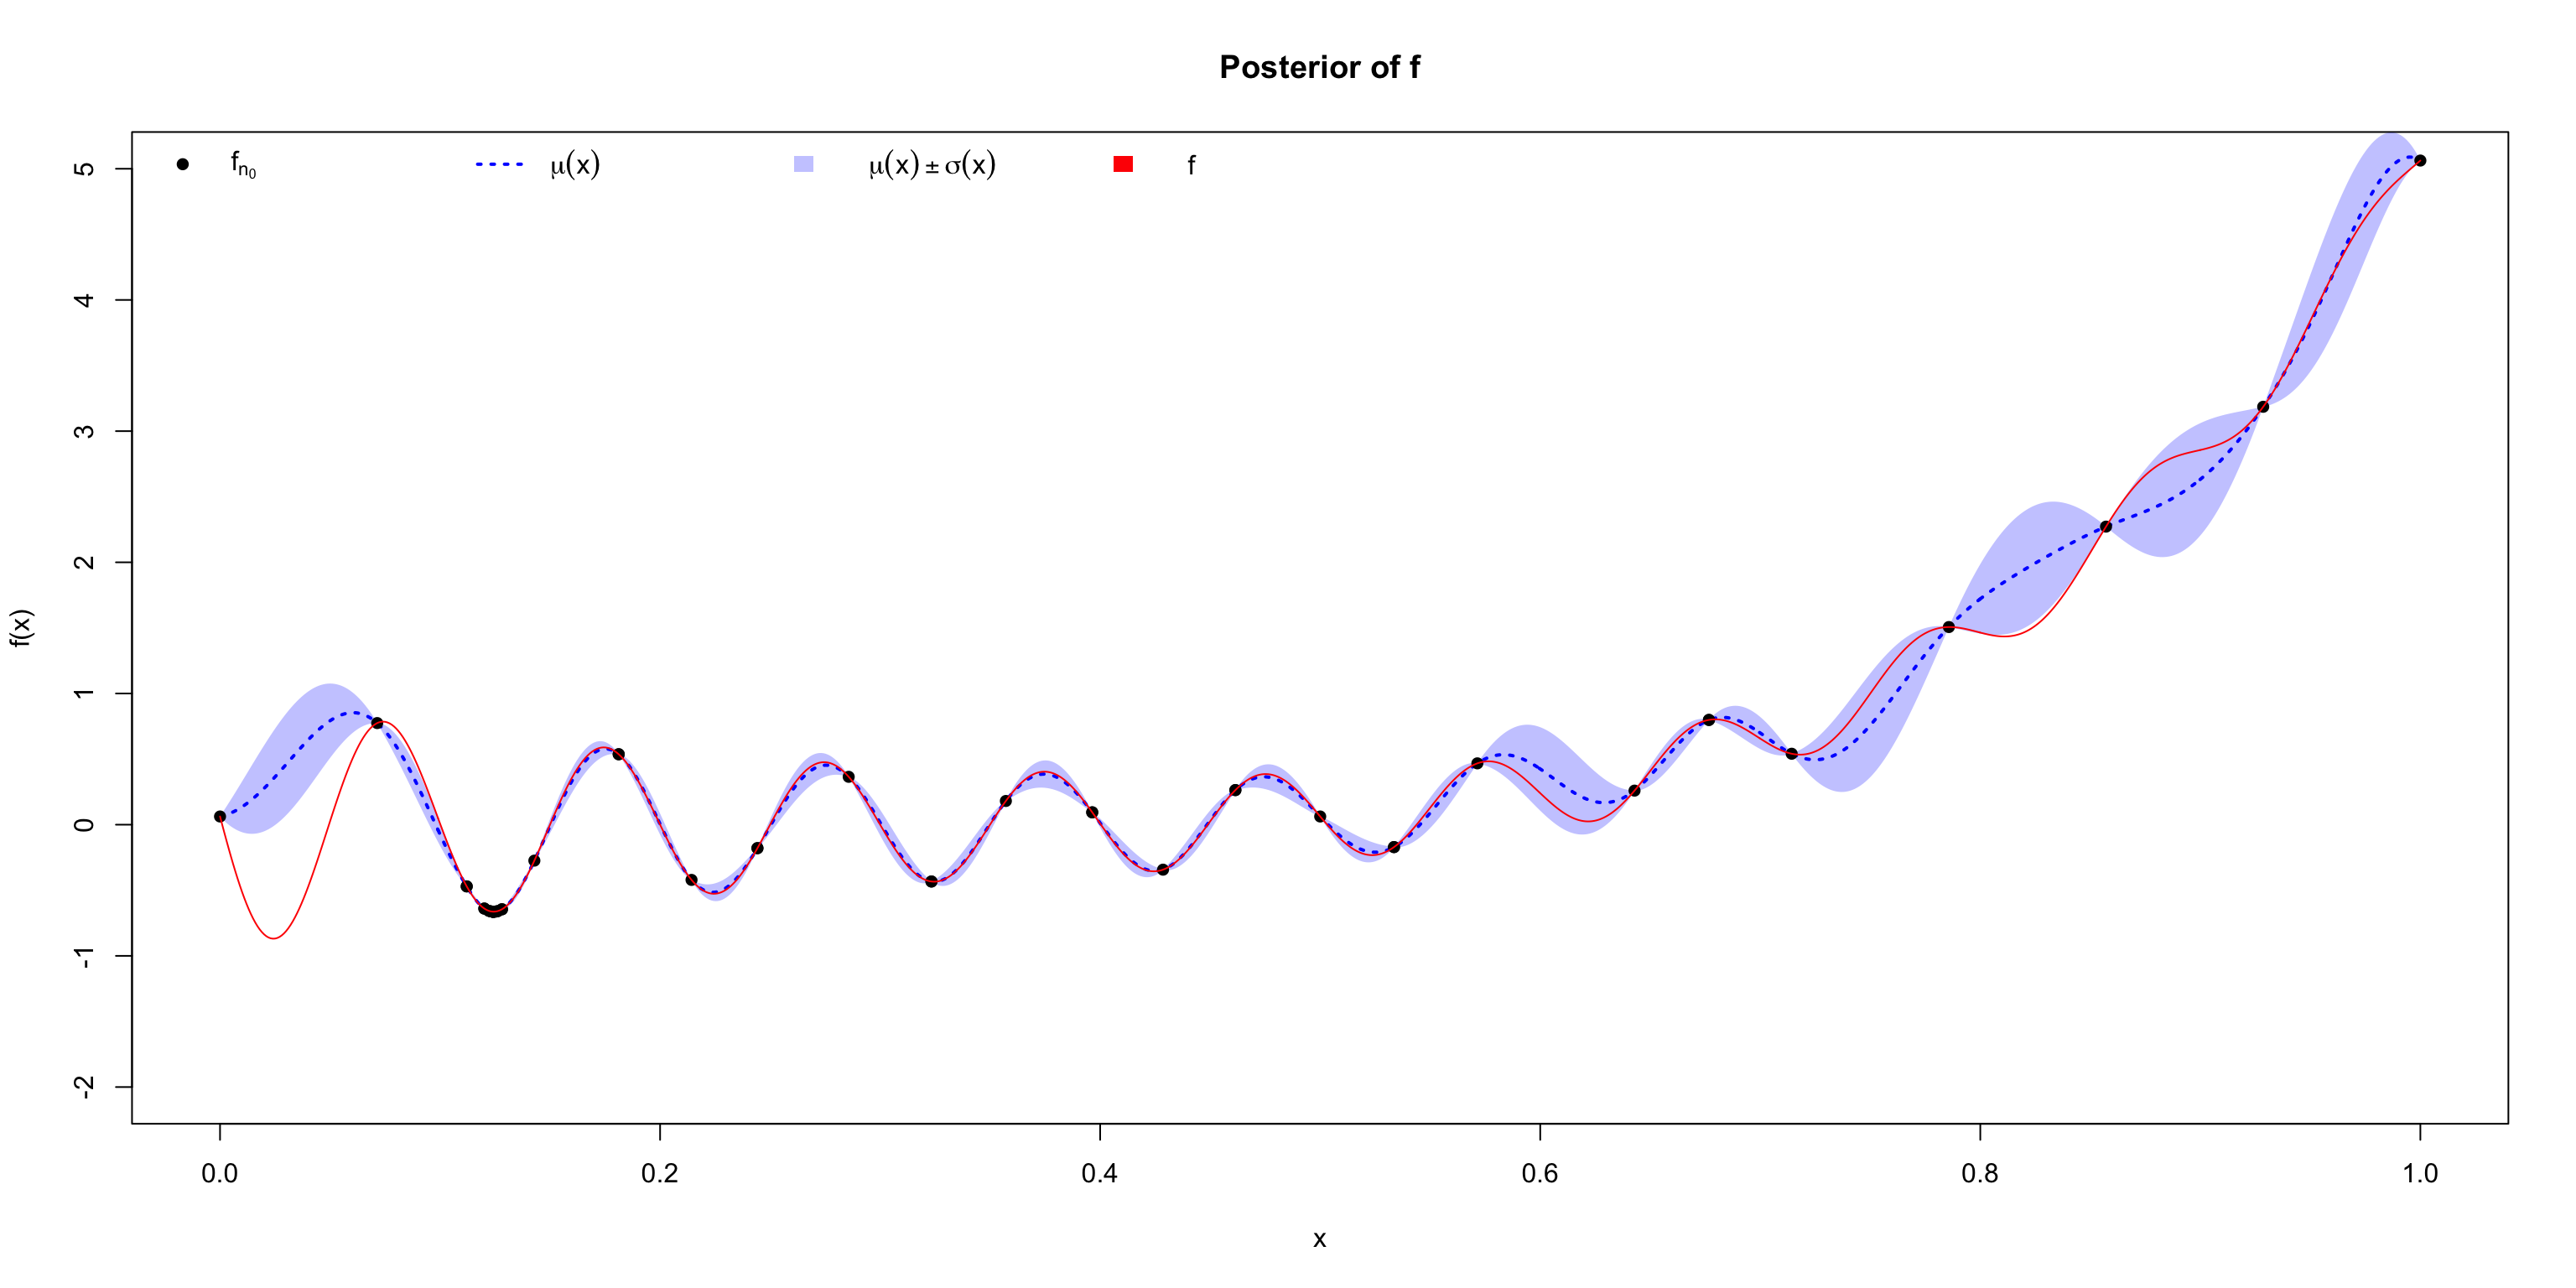
\includegraphics[width=1\textwidth]{Figures/45iter.png}
    \label{fig:45iter}
  \end{figure}
\end{frame}

\section{BASS}
\begin{frame}
  \frametitle{BASS}
  Los modelos BASS son una extensión de los modelos MARS, que hacen regresión lineal a pedazos. BASS se basa en RJMCMC para calcular la mejor distribución. 
  \newline \\
  Modelamos $y_i$ como sigue:
    $$ y_i = f(\boldsymbol{x}_i) + \epsilon_i, \, \, \epsilon_i \sim \mathcal{N}(0,\sigma^2) $$
    $$ f(\boldsymbol{x}) = a_0 + \sum_{m=1}^{M} a_m B_m(\boldsymbol{x}) $$
    $$ B_m(\boldsymbol{x}) = \prod_{k=1}^{K_m} g_{km} [s_{km}(\boldsymbol{x}_{v_{km}} - t_{km}) ]^\alpha_+ $$
\end{frame}

\begin{frame}
  \frametitle{Después de 45 iteraciones}
  Usamos BASS porque: 
  \begin{itemize}
      \item No es necesario que $f$ sea continua, puede ser discreta o categórica. 
      \item Puede ser lineal, o de grado $n$. 
      \item Mucho más ajustable que procesos Gausianos. 
  \end{itemize}
  Trade-offs: 
  \begin{itemize}
      \item Procesos Gausianos es óptimo. 
      \item Mucho más lento. 
  \end{itemize}
\end{frame}

\begin{frame}
  \frametitle{BASS inicial}
  \begin{figure}[h]
    \centering
    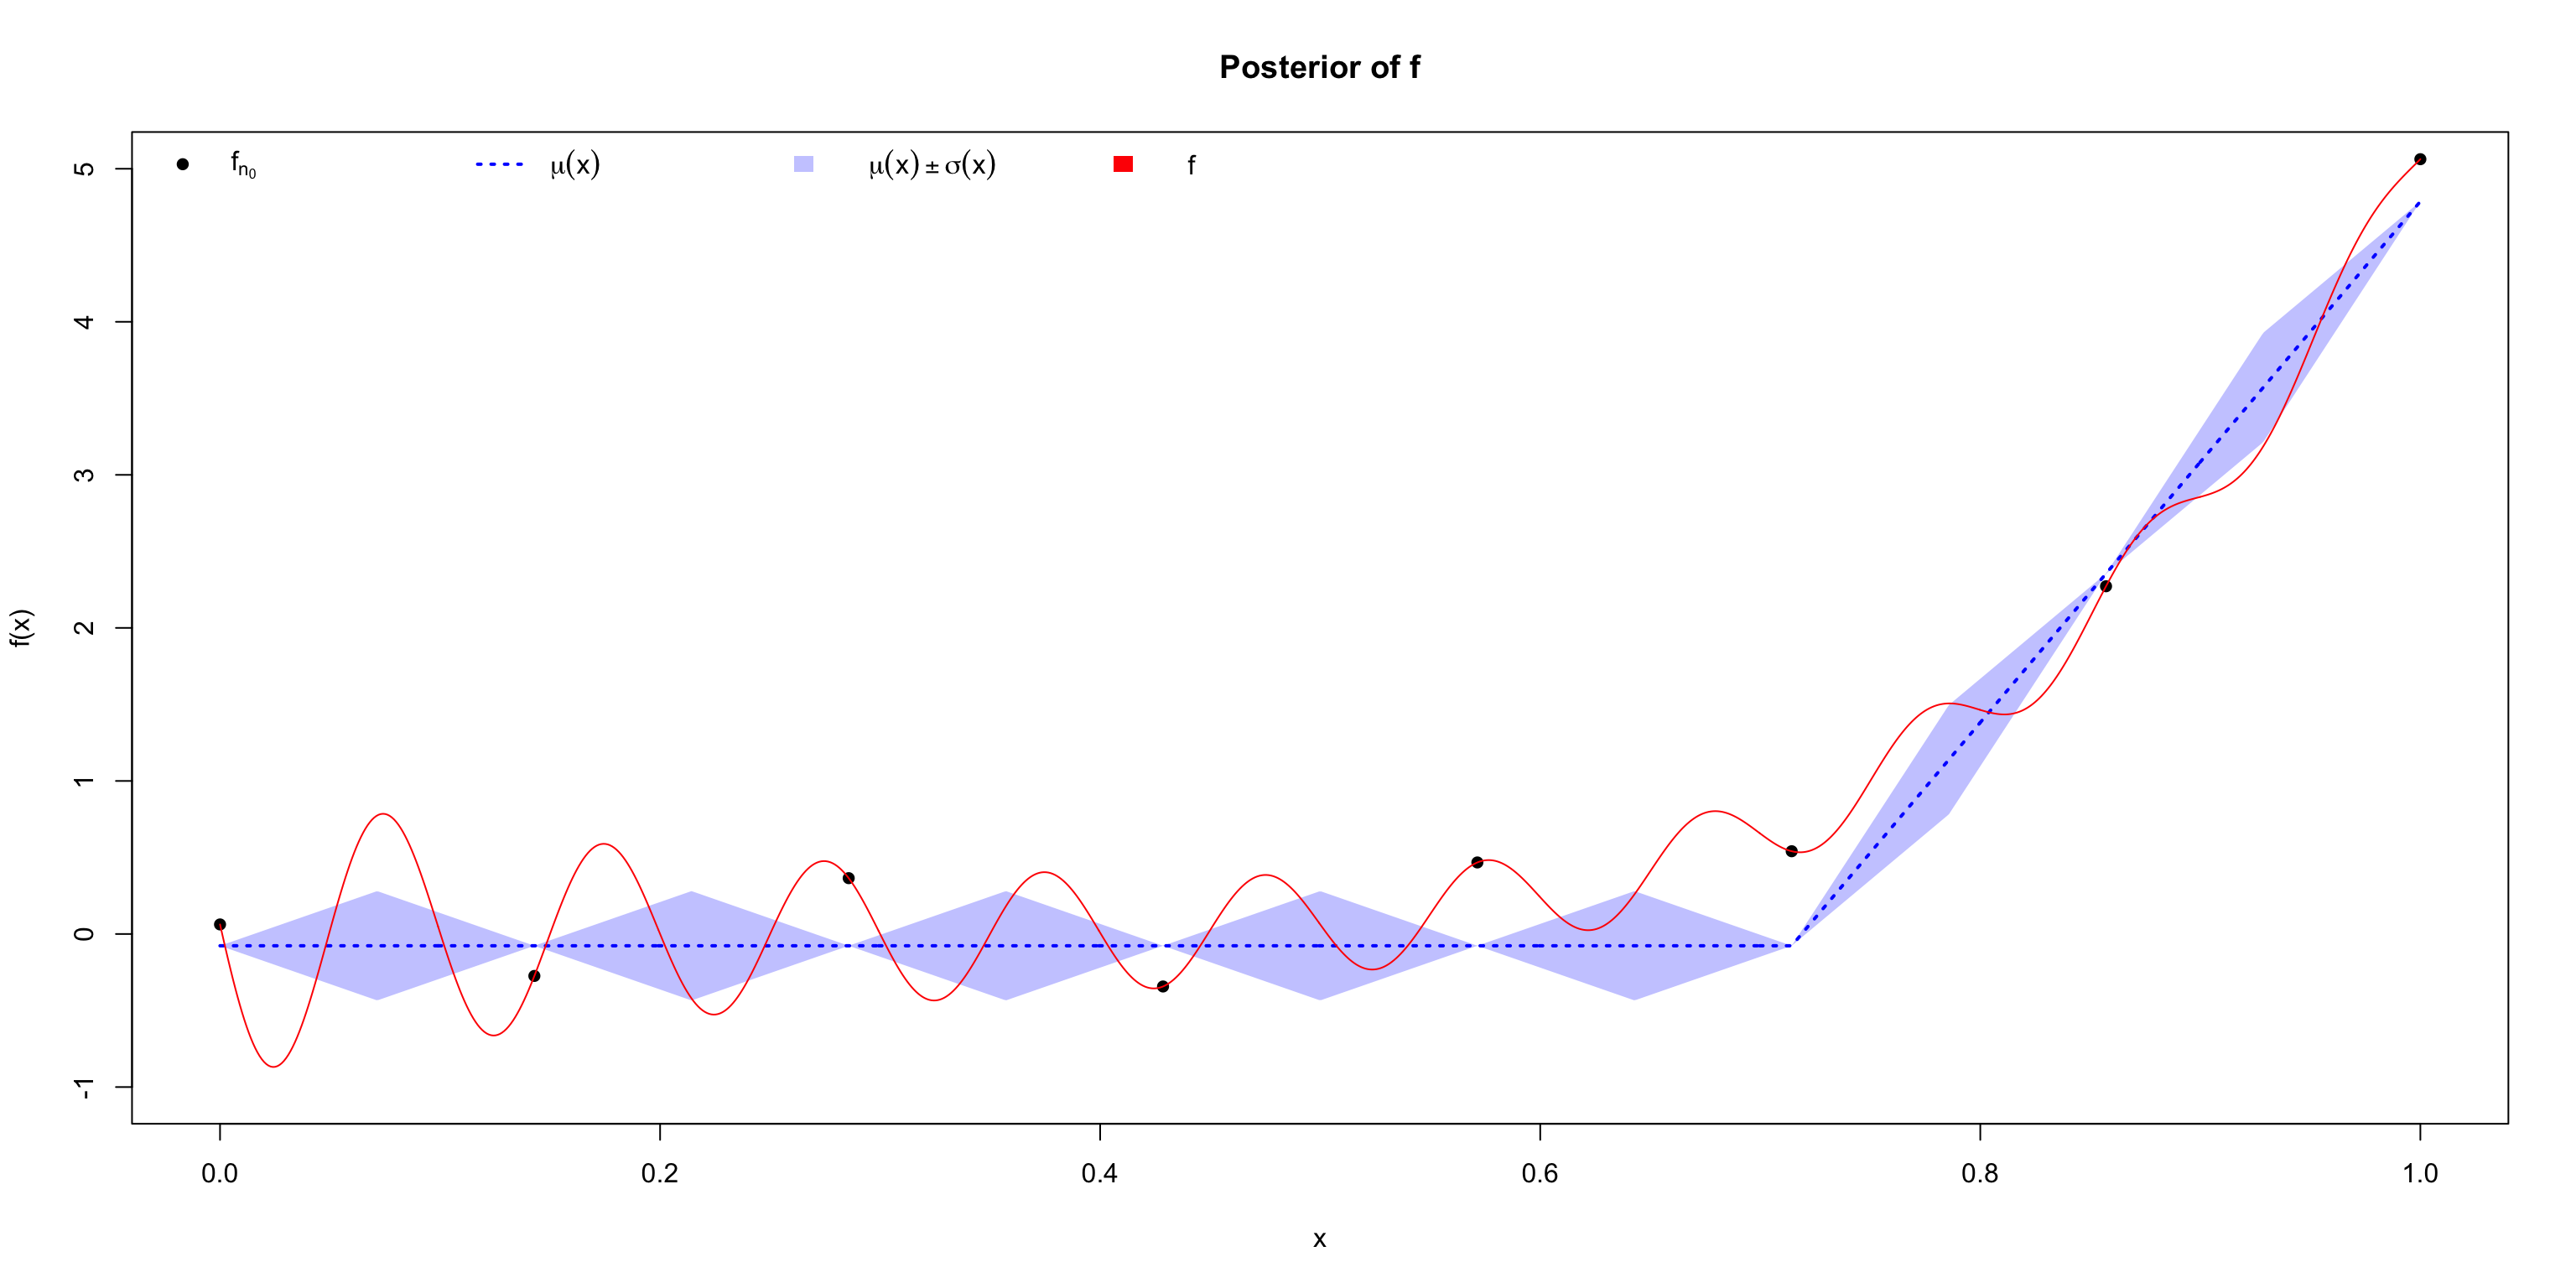
\includegraphics[width=1\textwidth]{Figures/BASS8.png}
    \label{fig:bass8}
  \end{figure}
\end{frame}

\begin{frame}
  \frametitle{BASS después de 115 iteraciones}
  \begin{figure}[h]
    \centering
    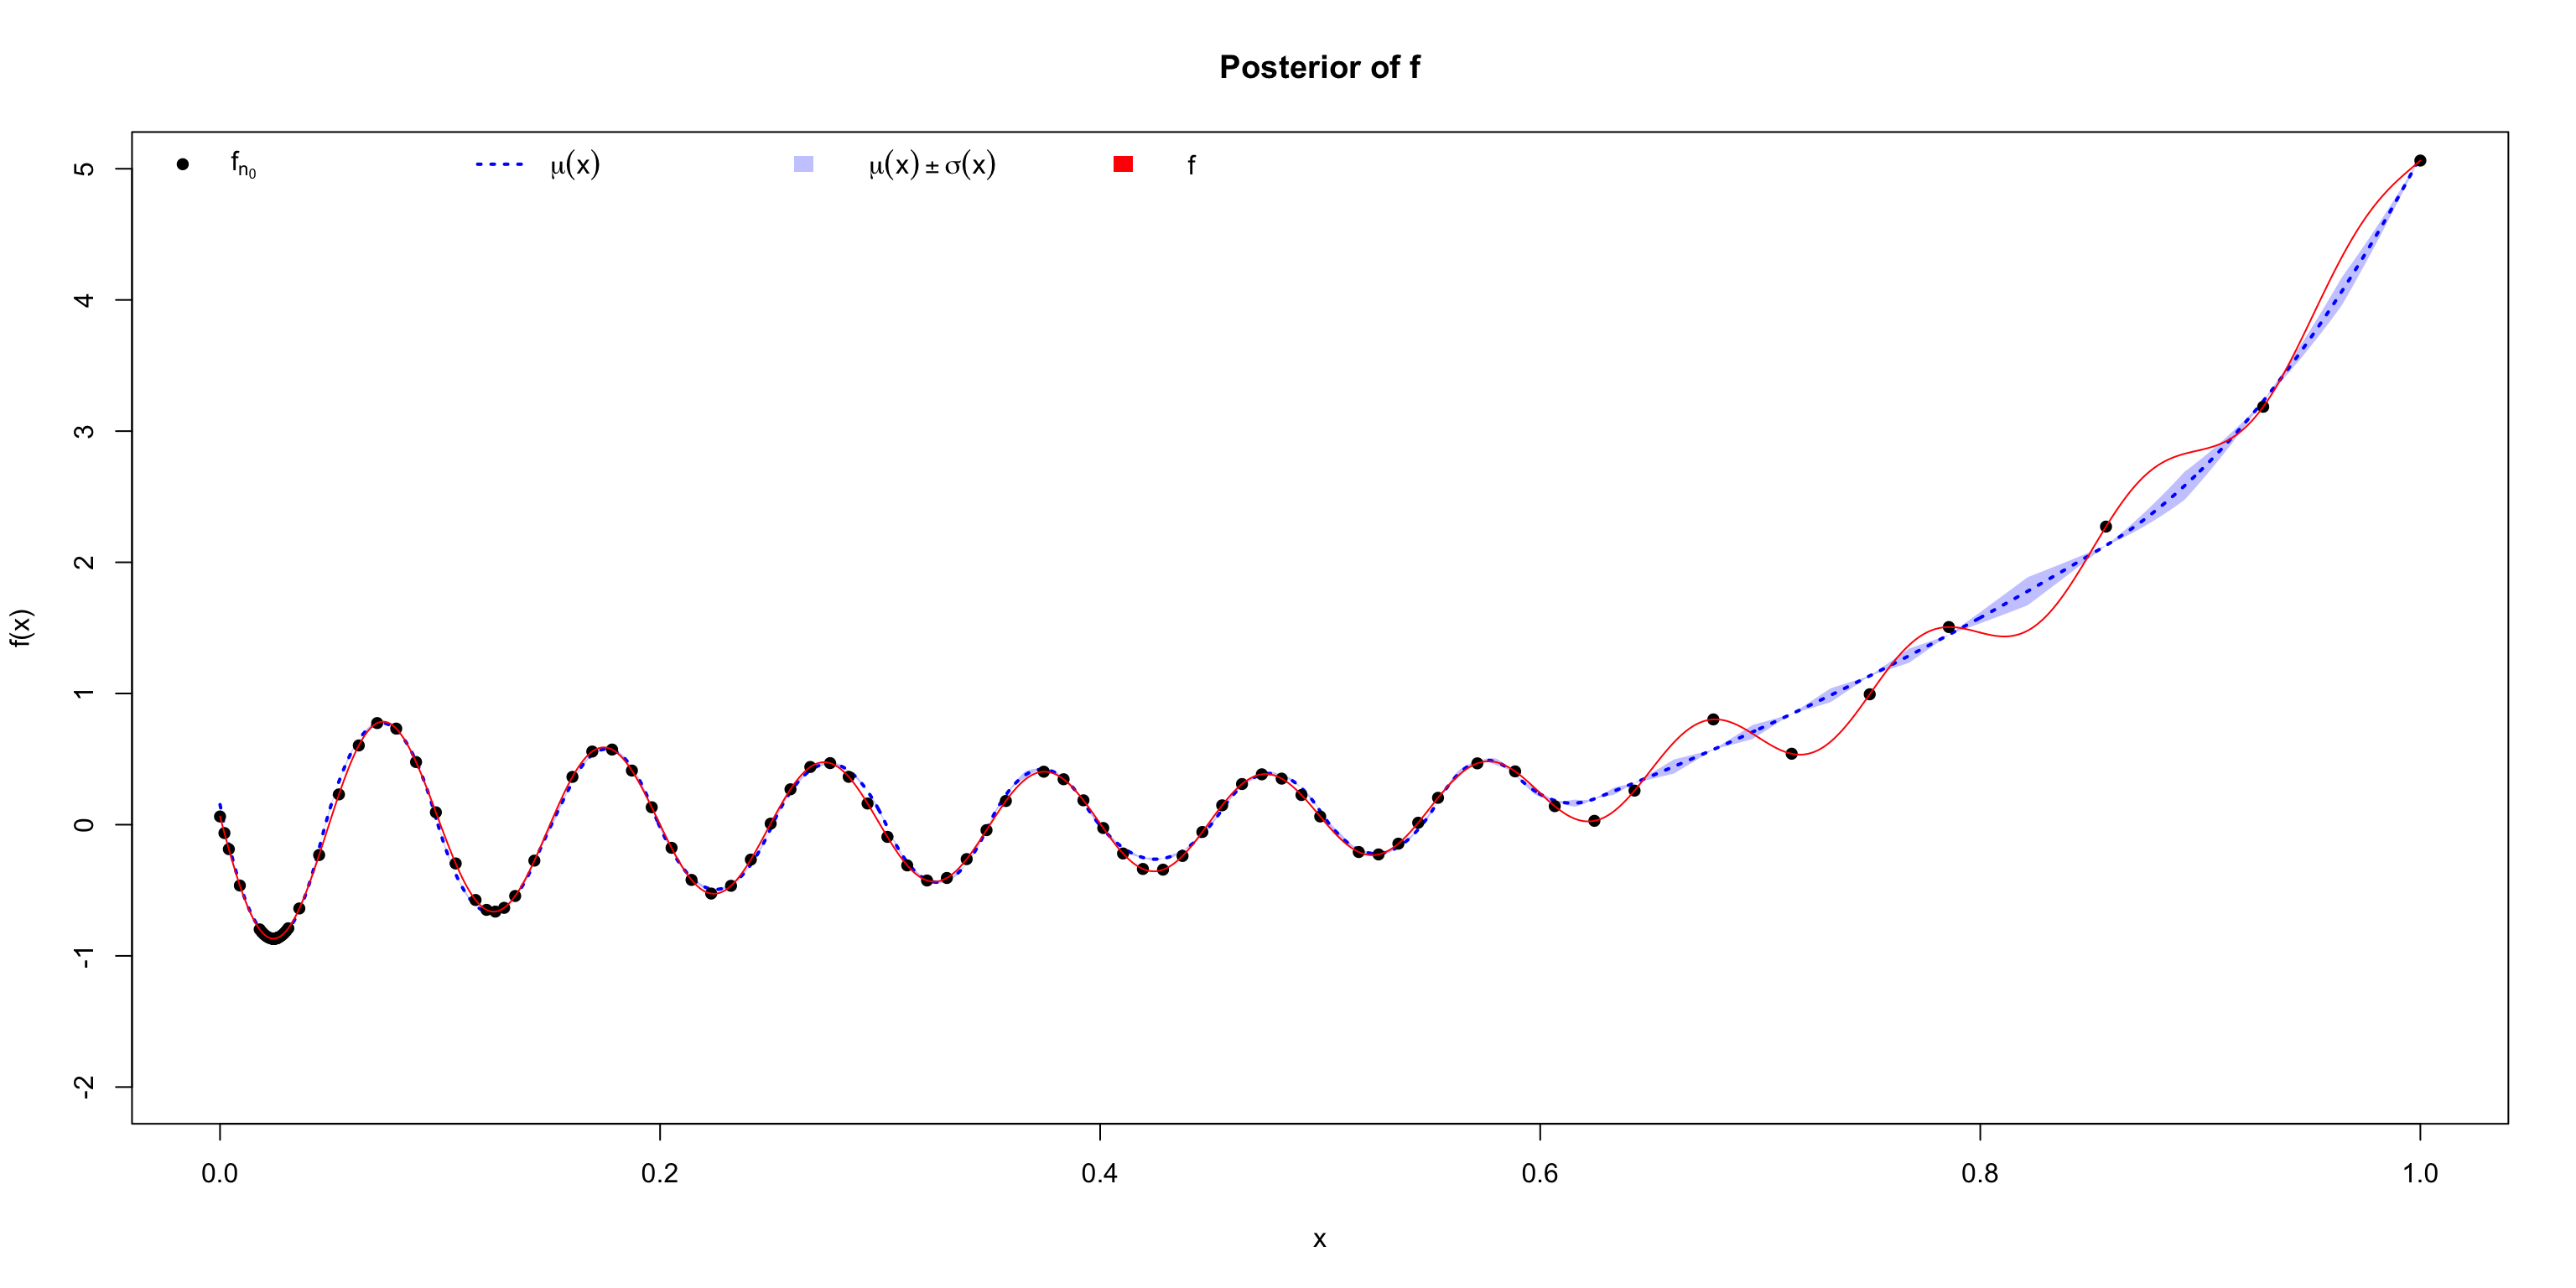
\includegraphics[width=1\textwidth]{Figures/115bass.png}
    \label{fig:bass115}
  \end{figure}
\end{frame}

\begin{frame}
  \frametitle{Problema real}
  \begin{figure}[h]
    \centering
    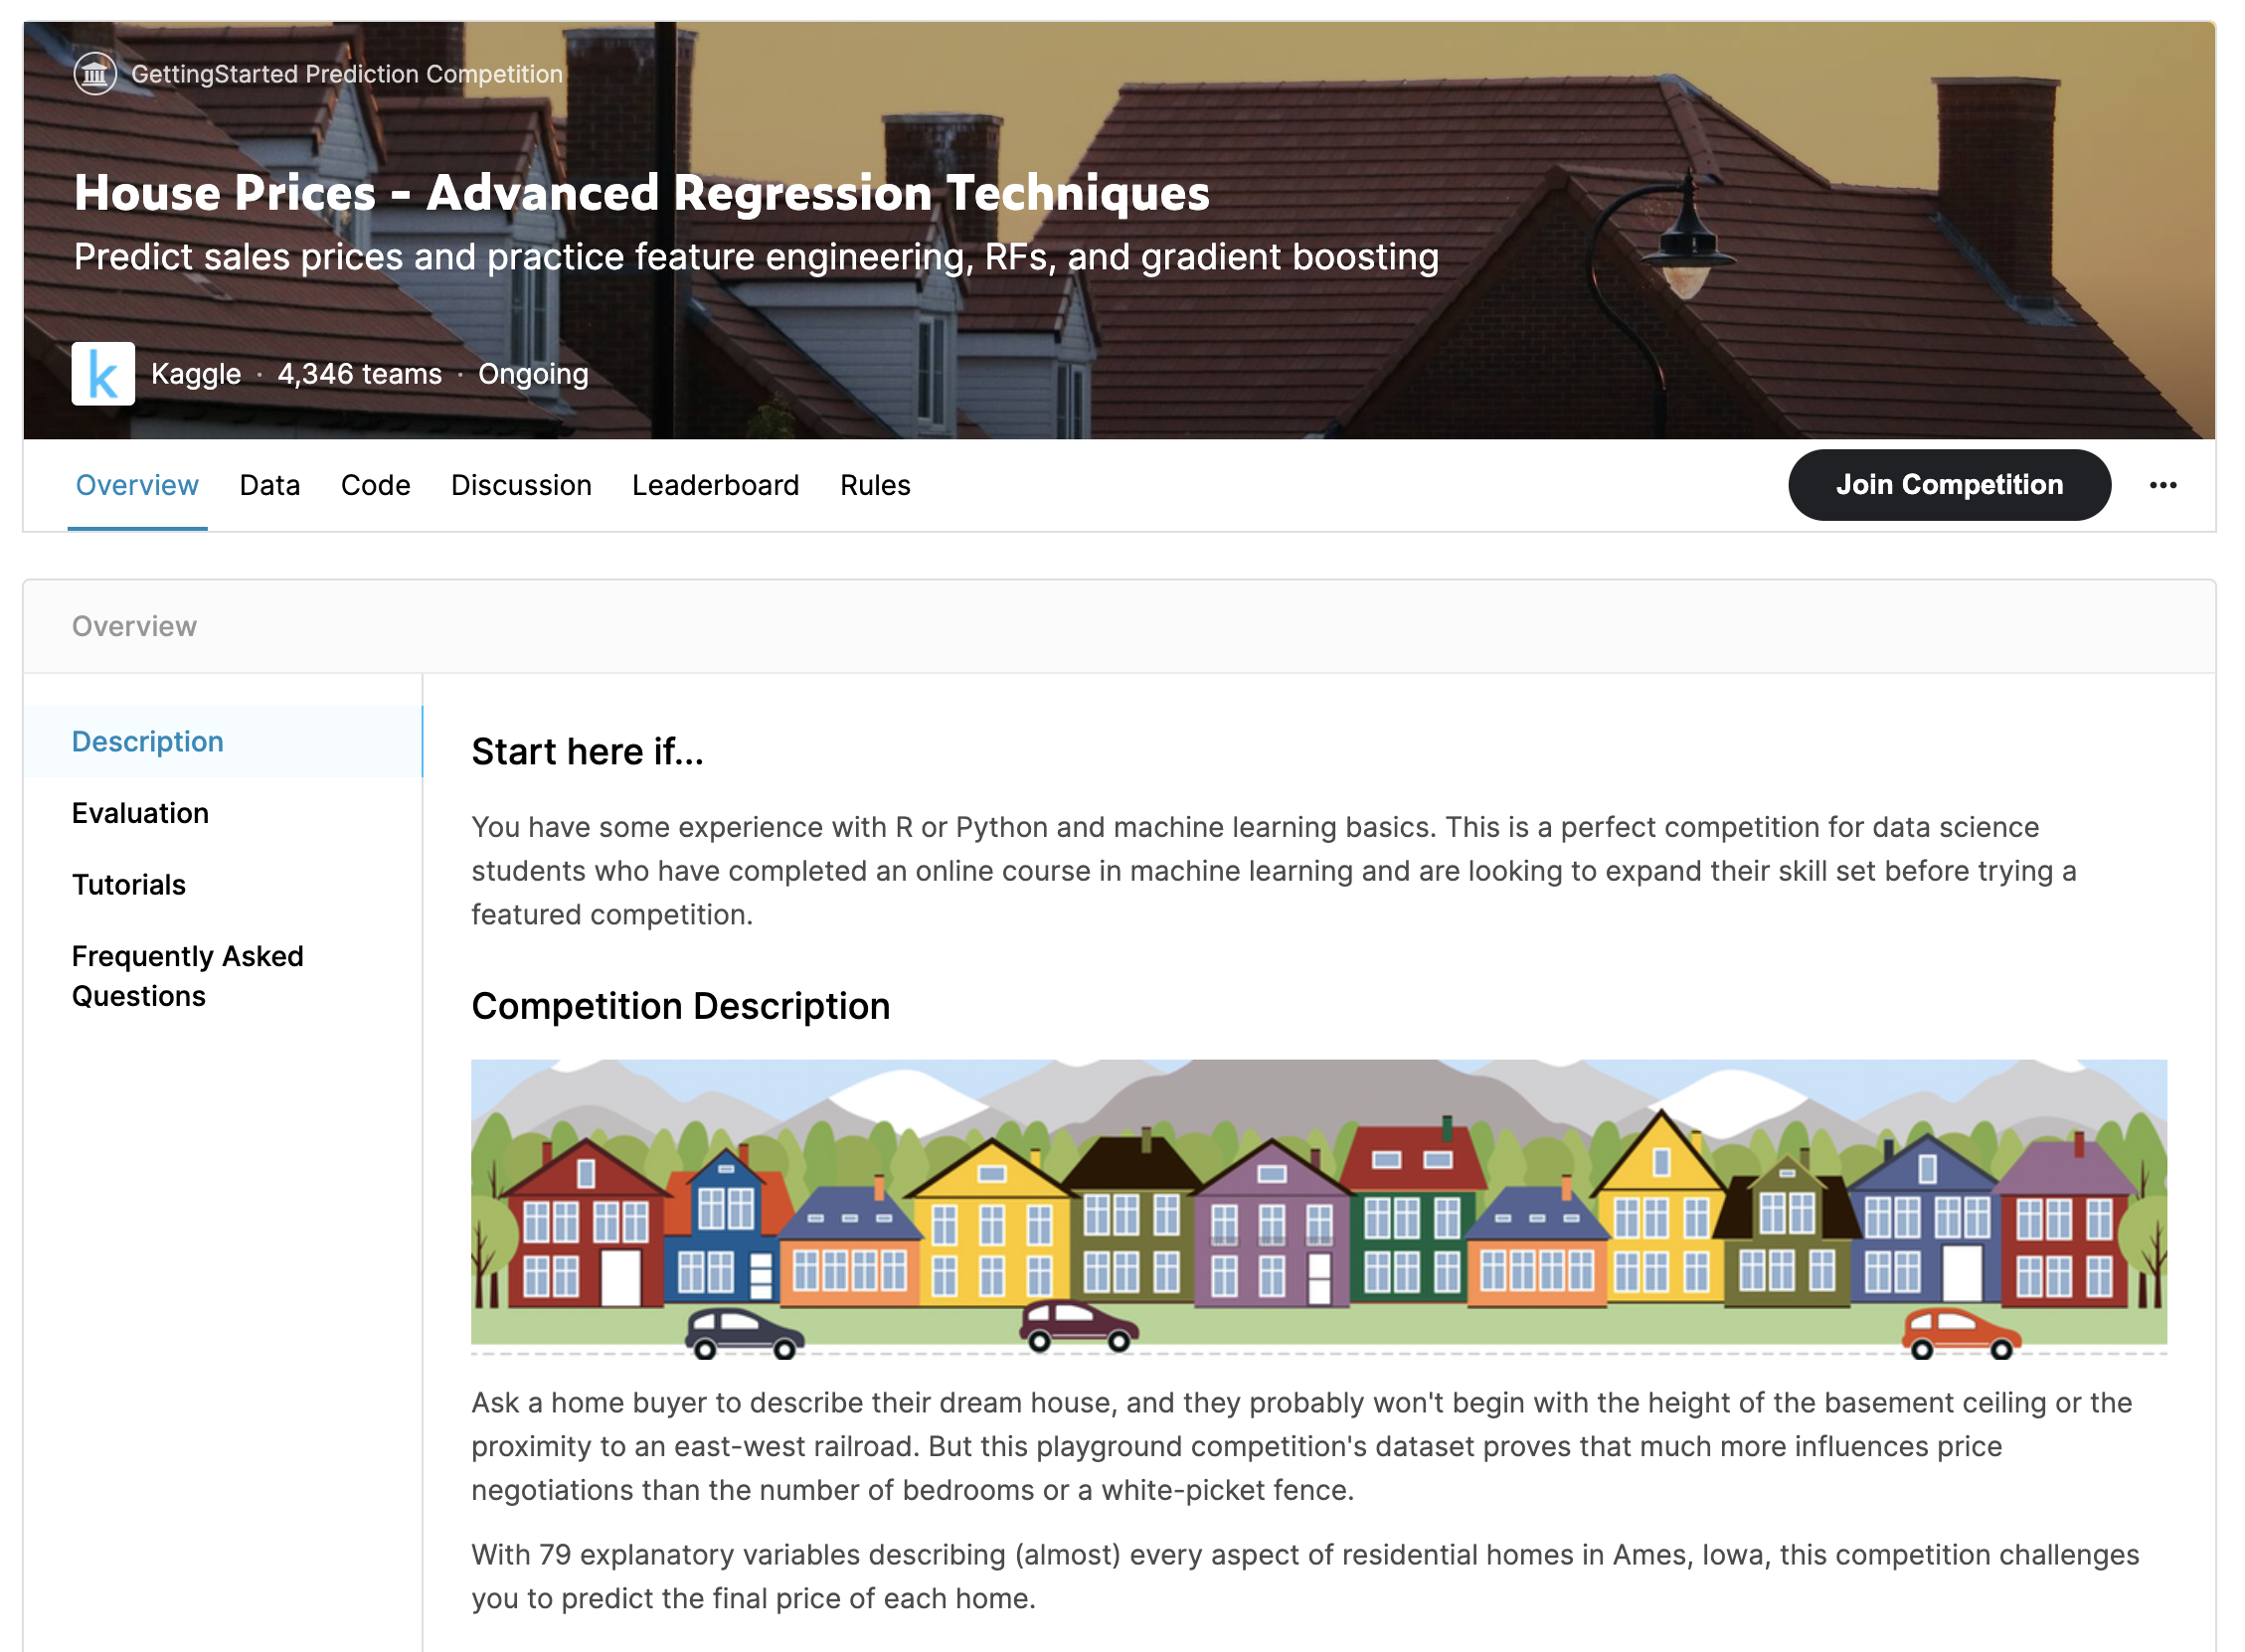
\includegraphics[width=1\textwidth]{Figures/ames.png}
    \label{fig:ames}
  \end{figure}
\end{frame}

\begin{frame}
  \frametitle{Problema real}
  Queremos ajustar un modelo \textit{elastic net}, de regresión regularizada, cuyos coeficientes se ven como sigue: 
  $$\hat \beta = \argmin_{\beta} ||y - \boldsymbol{X} \beta||^2 + \lambda \left( (1 - \alpha) ||\beta||_2^2 + \alpha||\beta||_1 \right).$$
  Sabemos que $\alpha \in [0,1]$, pero, ¿cual es la mejor $\alpha$ para minimizar el error?
\end{frame}

\begin{frame}
  \frametitle{Resultados de BASS}
  \begin{figure}[h]
    \centering
    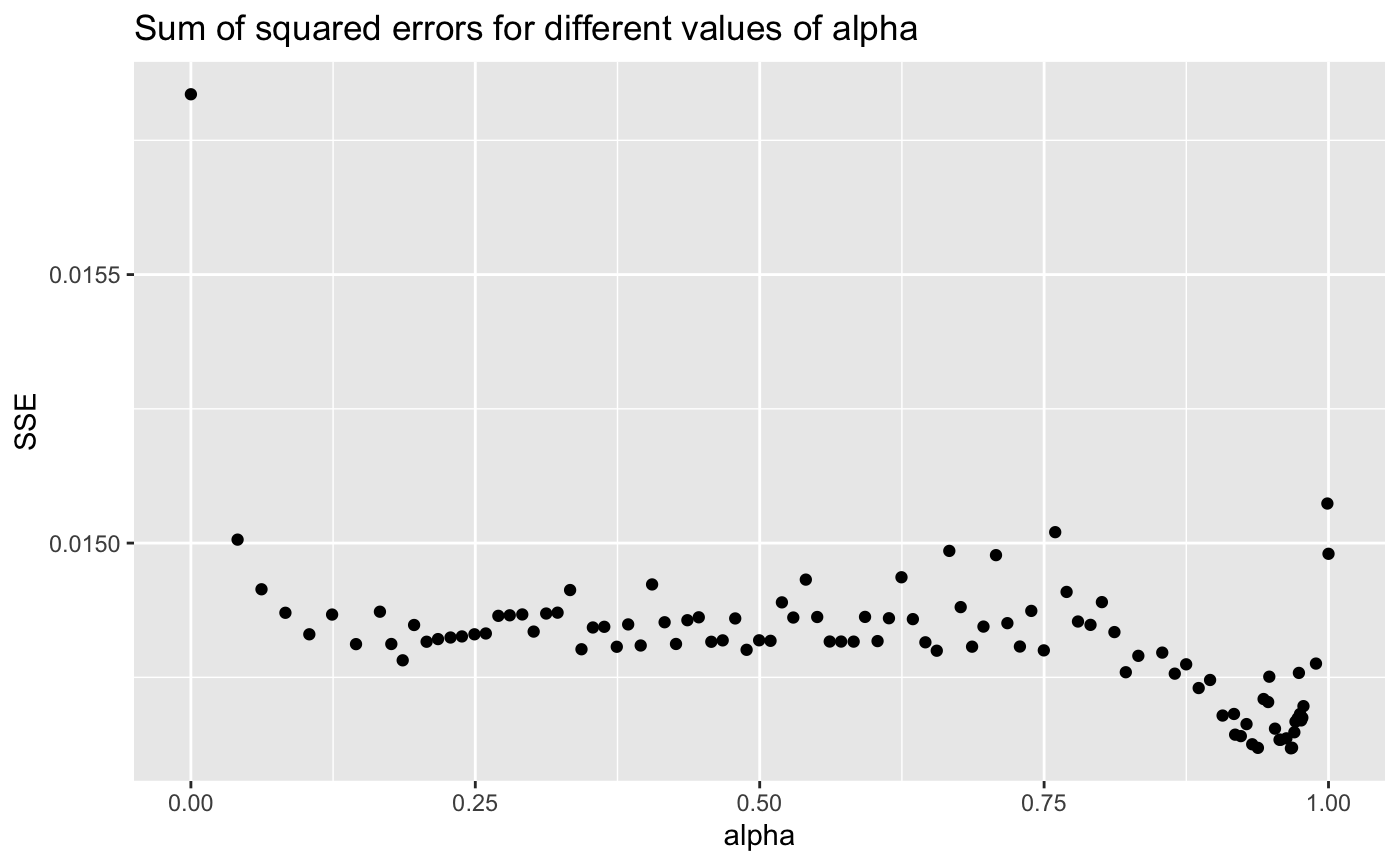
\includegraphics[width=1\textwidth]{Figures/sse_alpha.png}
    \label{fig:alfa}
  \end{figure}
\end{frame}

\begin{frame}
  \frametitle{Resultados de BASS}
  \begin{figure}[h]
    \centering
    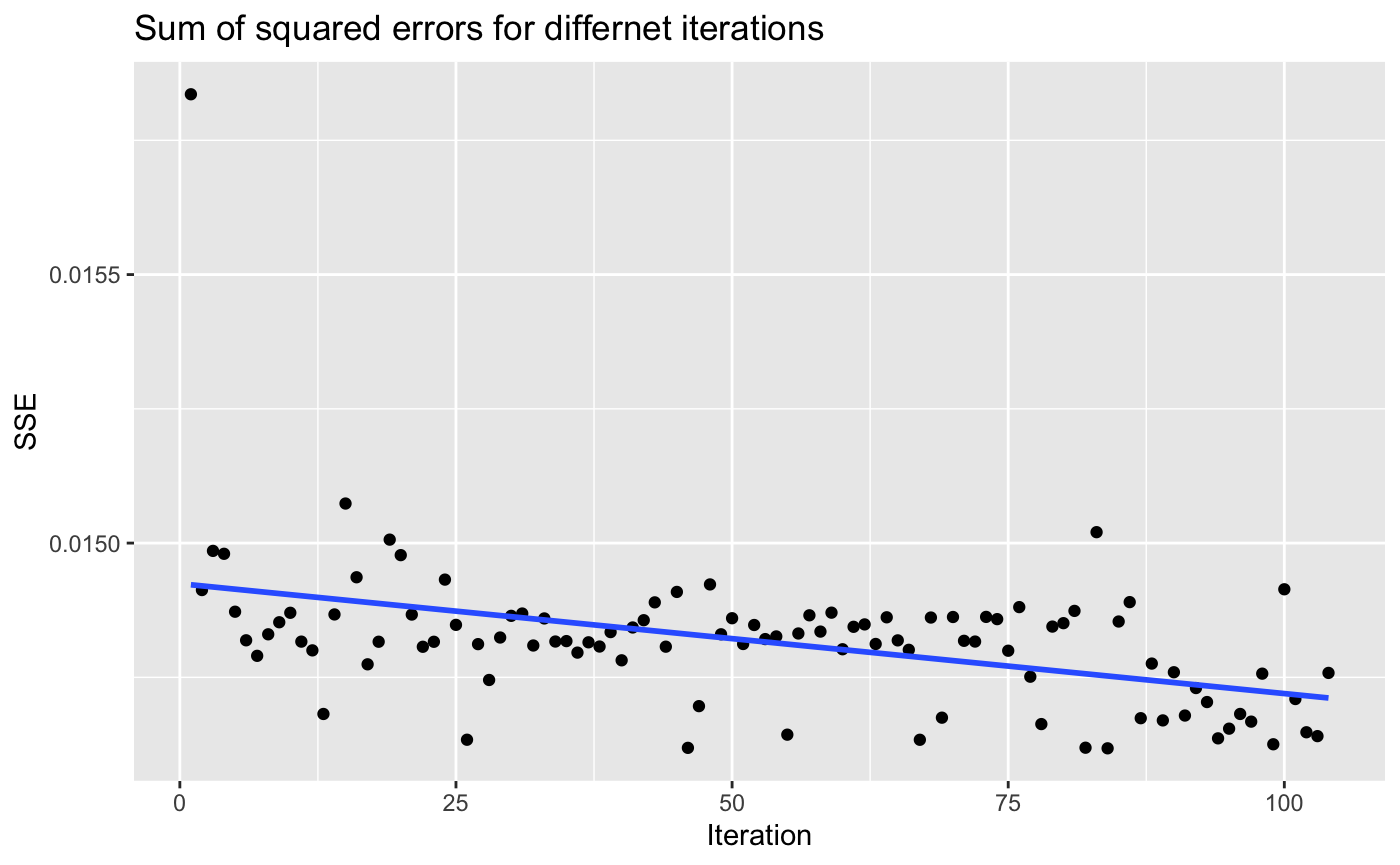
\includegraphics[width=1\textwidth]{Figures/sse_iter.png}
    \label{fig:iter}
  \end{figure}
\end{frame}

\end{document}